
\section{Introduction to CUBE ProjectAssistant} % Major section
% Example citation \cite{Figueredo:2009dg}. (Literaturangabe; Literaturliste)

In this tutorial, the short form CUBE PA will be used.

\subsection{What's the purpose of CUBE PA?} % Sub-section

CUBE PA is a tool for project management. As a database application with web-based access, it can be used at any time with any Internet connection. It supports typical work-flows such as meetings and procurements for the project management. It also makes all project management-relevant information available everywhere and at any time.

\subsection{Who should use CUBE PA?} % Sub-section

CUBE PA is particularly useful for projects with some of the following characteristics:

% \begin{itemize} % - Zu grosser Abstand verwendet
% 	\item xy
% \end{itemize}
	
\begin{compactitem}
	\item Several involved parties, companies, organizations
	\item The stakeholders are active in different workplaces
	\item Complex structure with many sub-projects
	\item Longer durations
	\item Big quantities of meetings, procurements, etc.
	\item Time difference between the stakeholders
	\item Need for flexible work possibilities outside the office, on the train, day and night, etc.
\end{compactitem}	
		
\ \\
If a project is chosen for using CUBE PA, it is of central importance that all persons involved in project management use CUBE PA. This concerns both the decision-makers and their assistants. This is the only way to achieve the maximum benefit from the initial effort required to set up CUBE PA.
	
\subsection{The CUBE PA structure} % Sub-section

CUBE PA is divided into the different fields described below, each corresponding to a menu item. The development of the fields is currently unequal, some fields being well developed, others being still rudimentary. Further fields are also planned. Each field is briefly described below in order to give the reader a clue as to its intended use and its state of development. A separate chapter further below describes how each field can be used.

\pagebreak
\subsubsection{The CUBE PA menu} % Sub-sub-section

\setlength{\abovecaptionskip}{0pt}

\begin{wrapfigure}[16]{l}{7cm}   % [x] Wie manche Zeile soll sich um die Grafik "brechen"
  \vspace{-25pt}      % Grundwert war 20; mit 30 schön oben beim Text ausgerichtet
  \begin{center}
    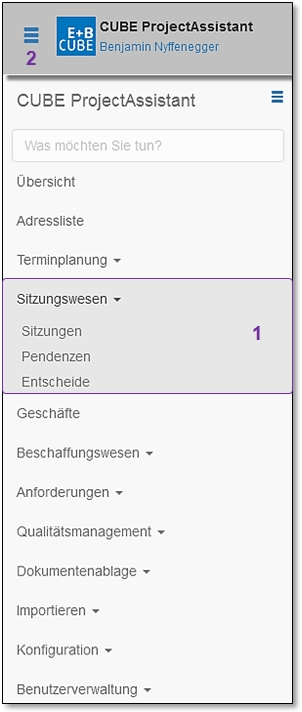
\includegraphics[height=150mm]{../chapters/01_Einfuehrung/pictures/1-3-1_Menuuebersicht_oSitzungswesen.jpg}
  \end{center}
  \vspace{-20pt}
  \caption{The menu}
  \vspace{-10pt}
\end{wrapfigure}
The various fields of CUBE PA can be accessed at any time via the menu. Depending on the field, you can choose between different subcategories. To do so, click on the desired menu item. If there are further subcategories, these are also displayed. Under the „Meeting Management“ \col{(1)} menu item, the three sub-items „Meetings“, „Actions“ and „Decisions“ are displayed. Clicking on the desired sub-item opens it. Clicking again on the main menu item („Meeting Management“) hides the sub-items.

\vspace{\baselineskip}

By clicking on the menu icon \col{(2)} you can show and hide the menu. This way a larger work area is available for you to use. \\

\vspace{6.5cm}  

\textbf{Customized menu}

\begin{wrapfigure}[7]{r}{5.5cm}
\vspace{-35pt}
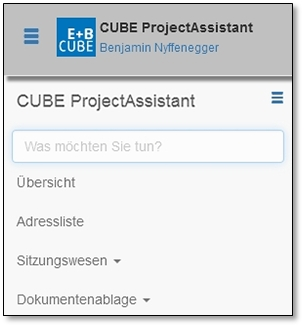
\includegraphics[height=60mm]{../chapters/01_Einfuehrung/pictures/1-3-1_MenuAngepasst.jpg}
\caption{Customized menu}
\end{wrapfigure}

The different menus and menu items shown in the screen shots in this tutorial may differ between users according to the authorizations given to them (different roles, e.g. administrator). In this tutorial, all menu items are shown.

\subsubsection{Overview}
\label{bkm:Ref132000001}
The personal project overview is the first thing to appear when you log in to CUBE PA. It gives you a quick overview of the issues you are directly concerned with.

\begin{figure}[H] % Example image
\center{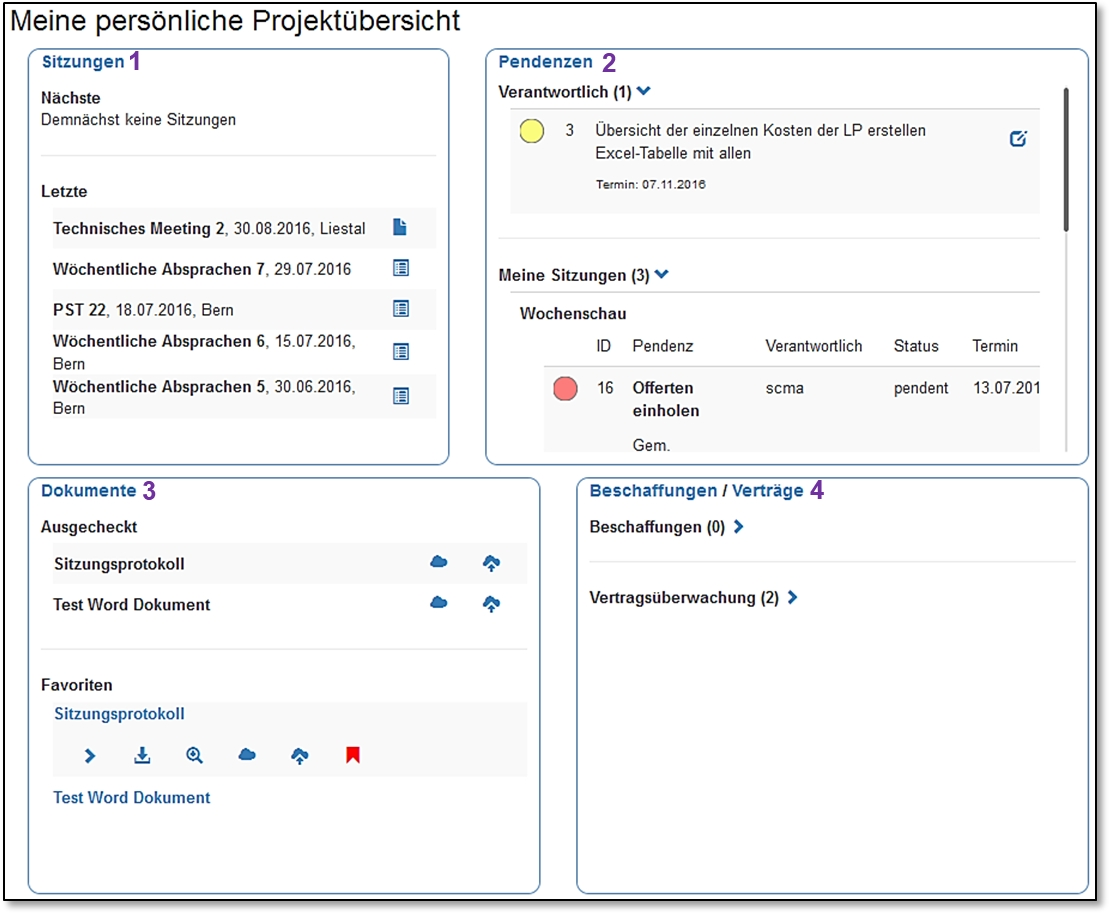
\includegraphics[width=1\linewidth]{../chapters/01_Einfuehrung/pictures/1-3-2_persUebersicht.jpg}}
\caption{My personal project overview}
% \label{fig:speciation}
\end{figure}

At the top left, the current meetings are shown \col{(1)}. Under „Next“, upcoming meetings in which you are a participant are shown. You can edit a meeting or save it as a PDF file. Under „Past“, meetings which have recently been held are shown. Click to open the meeting minutes. If there are no finalized meeting minutes available, you can edit them. Click on the blue title „Meetings“ \col{(1)} to go directly to the „Meetings“ subcategory in the „Meeting Management“ field.

\vspace{\baselineskip}

At the top right, the actions \col{(2)} for which you are responsible or whose execution concerns you (collaboration) are shown. Click on an action to edit it. The corresponding form will be opened. Click on the blue title „Actions“ \col{(4)} to go directly to the „Actions“ subcategory in the „Meeting Management“ field. Refer to chapter 5.4 for creating actions and to chapter 5.5 for editing actions.

\vspace{\baselineskip}

At the bottom right, the relevant documents \col{(3)} are displayed. Under „Checked-out“, documents you have checked-out are displayed. You have the option to open or to check-in a checked-out document. \\

Under „Favourites“, the documents you have marked as personal favourites are listed. Click on a listed document title to display the options: you can download the document, view its details, change the entry, or check-out the document to edit it while it's blocked for other users. You can also view a preview of the document. If you no longer need a document as a favourite, click on the red flag symbol. The the entry disappears after updating the view or by clicking on 'Dashboard'. If you click again on the document title, the options are hidden. Click on the blue title „Documents“ \col{(3)} to go directly to the „Documents“ subcategory in the „Document Management“ field.

\vspace{\baselineskip}

% Text, welcher bis zur Grafik reichen soll, ist unmittelbar an Grafikeinbettung 
% zu schreiben, dann kommt Grafikeinbettung, dann Text, welcher Grafik umschliesst.

\begin{wrapfigure}{r}{0.5\textwidth}
  \vspace{-20pt}
  \begin{center}
    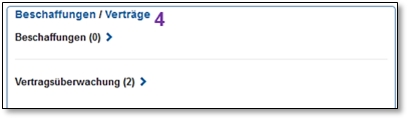
\includegraphics[width=0.5\textwidth]{../chapters/01_Einfuehrung/pictures/1-3-2_persUebersichtBeschaffung.jpg}
  \end{center}
  \vspace{-20pt}
%  \caption{Persönliche Übersicht}
  \vspace{-10pt}
\end{wrapfigure}
At the bottom right, procurements and contracts \col{(4)} in which you are involved and for which you need to take action are shown. The number of entries you are involved in is shown between brackets. Click on the horizontal arrow icon to show a procurement or contract. Click on the magnifying glass icon next to a procurement or contract to directly edit it. However, depending on the status of the procurement, it may be more appropriate to access the right processing option via the menu, using the „Procurement Function“ menu item and its subcategories. Refer to chapter 7 for a description of the procurement function. Click on the blue titles „Procurements“ or „Contracts“ \col{(4)}, to go directly to the subcategories „Procurements“ or „Contracts“ in the „Procurement Function“ field.

\vspace{\baselineskip}

\begin{wrapfigure}[5]{r}{0.5\textwidth}
  \vspace{-30pt}
  \begin{center}
    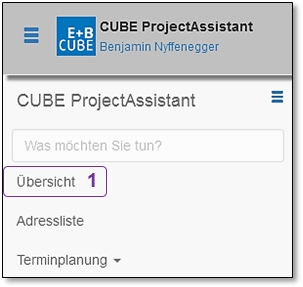
\includegraphics[width=0.4\textwidth]{../chapters/01_Einfuehrung/pictures/1-3-2_MenuepunktUebersicht.jpg}
  \end{center}
  \vspace{-20pt}
  \caption{Menu Overview}
  \vspace{-10pt}
\end{wrapfigure}
When you switch to a different field using the menu, you leave your personal overview. To return to your personal overview, click on „Dashboard“ \col{(1)} in the menu.

\pagebreak
\subsubsection{Address List} % Sub-sub-section

In the address list, all persons (users) and companies (participants) registered in CUBE PA are displayed in a simple way. Using the filter function, the desired entries can quickly be found.

\subsubsection{Scheduling} % Sub-sub-section

This functionality is currently rudimentary and is essentially limited to downloading documents. It is therefore not described in detail for the time being. 'Projectplans' is a Microsoft Project import (xml-file) which allows to filter and display the imported data.

\subsubsection{Meeting Management} % Sub-sub-section

CUBE PA supports the full work-flow for the loading and logging of meetings, with the exception of calender appointments and room bookings which are typically carried out in Outlook. The data recorded for a meeting is automatically available as a basis for the minutes of the meeting. The minutes can be directly recorded in CUBE PA and corrected by the participants.

\subsubsection{Transactions} % Sub-sub-section

CUBE PA supports a simple, structured project journal. If this is conscientiously managed, all project participants are always up-to-date, anytime and anywhere.

\subsubsection{Procurement Function} % Sub-sub-section

CUBE PA supports the complete work-flow of a procurement, from the tender publication to the tender and the tender inspection to the contract. The links between the tender publications, tenders and contracts are easy to observe thanks to an intelligent numbering system. For the time being, the functionality for procurements with only one tenderer (limited procedure) is implemented. The functionality for procurements with multiple tenderers follows in a next development step.

\subsubsection{Requirements} % Sub-sub-section

This functionality is currently rudimentary and is essentially limited to downloading documents. It is therefore not described in detail for the time being.

\subsubsection{Quality Management / Handbooks} % Sub-sub-section

This functionality is currently rudimentary and is essentially limited to downloading documents. The 'Handbooks' functionality allows the gathering of project handbooks or other handbooks in CUBE PA.

\subsubsection{Document Management} % Sub-sub-section

The document management enables the versioning of documents of all types. The stored documents can be identified with metadata / tags. In addition to the possibility to check-in and check-out documents and directly edit them in Office programs (as with Microsoft SharePoint), the documents can be viewed online (preview function). Each document can be assigned to a geographic location (by double-clicking directly in Google Maps). The location can later be changed in the map by drag and drop. The document management provides an overview of geographically close documents.

\subsubsection{Import} % Sub-sub-section

This option allows you to import projectplan and transactions data.

\subsubsection{Configuration} % Sub-sub-section

The configuration is used to enter project-specific data, which are then to be displayed in selection lists. This work must normally only be carried out by a few persons and is therefore only briefly described.

\subsubsection{User Management} % Sub-sub-section

Under User Management, the users, teams and groups are created and managed.
